\begin{figure}[!htbp]
\caption{Distribution of Legislator Ideal Points and District Ideology}
\begin{centering}
%\centering
%\fbox{
  \begin{tabular}{@{}ccc@{}}%{@{}ccc@{}}
	 & & \\  	
  	\small (A) Legislator Ideal Point & 
  	\small (B) Legislator Ideal Point (Key Votes) & 
  	\small (C) Ideal Point Comparison \\
    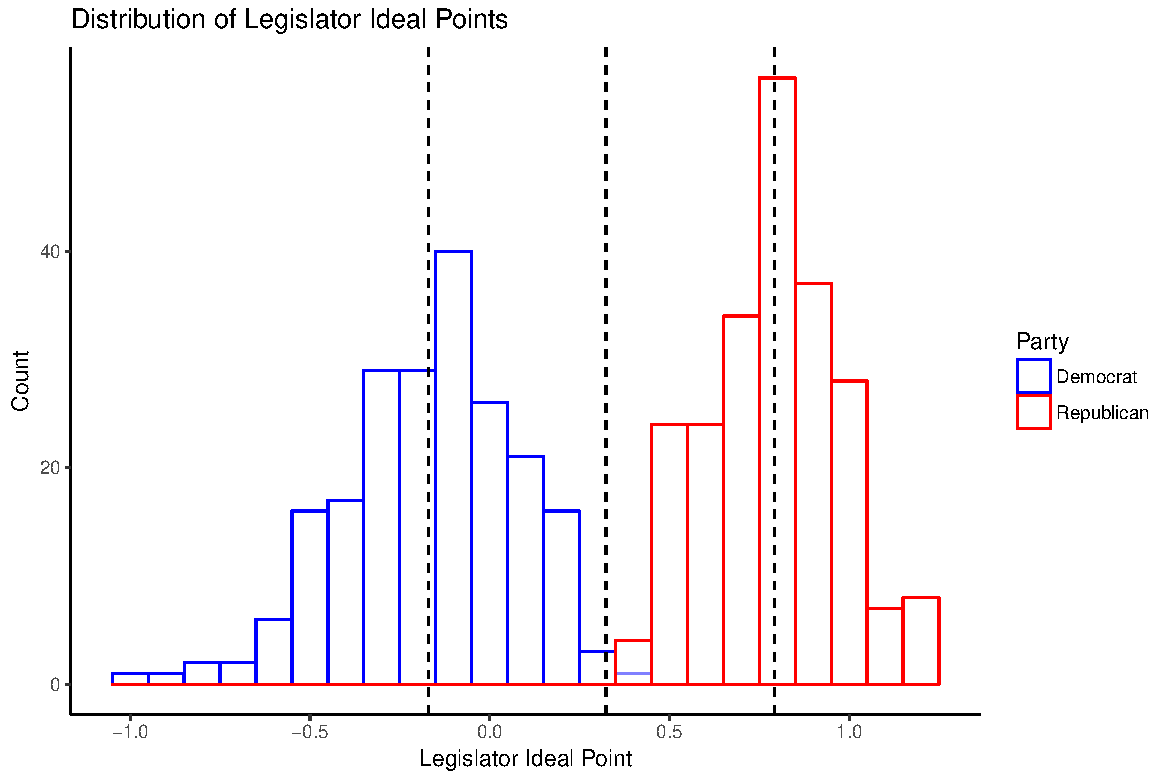
\includegraphics[width=.33\textwidth]{/Users/dsimp/GitHub/Clinton(2006)Rep/drafts/histogram/histogram-1} &
    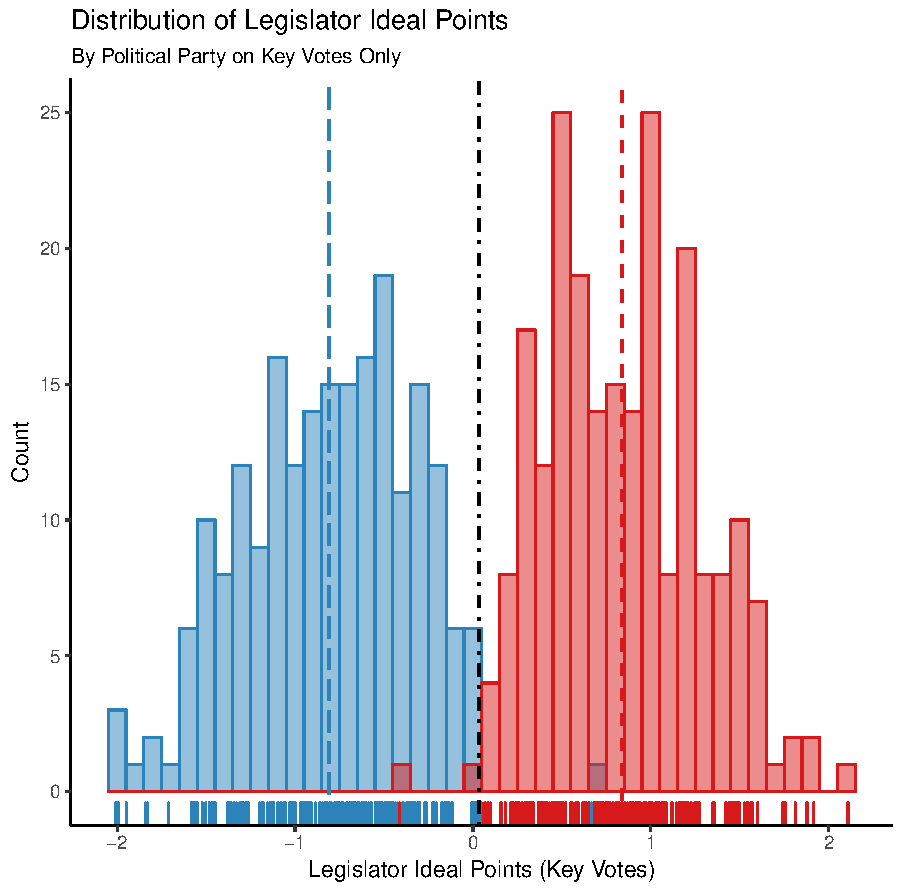
\includegraphics[width=.33\textwidth]{/Users/dsimp/GitHub/Clinton(2006)Rep/drafts/histogram/histogram-2} &
    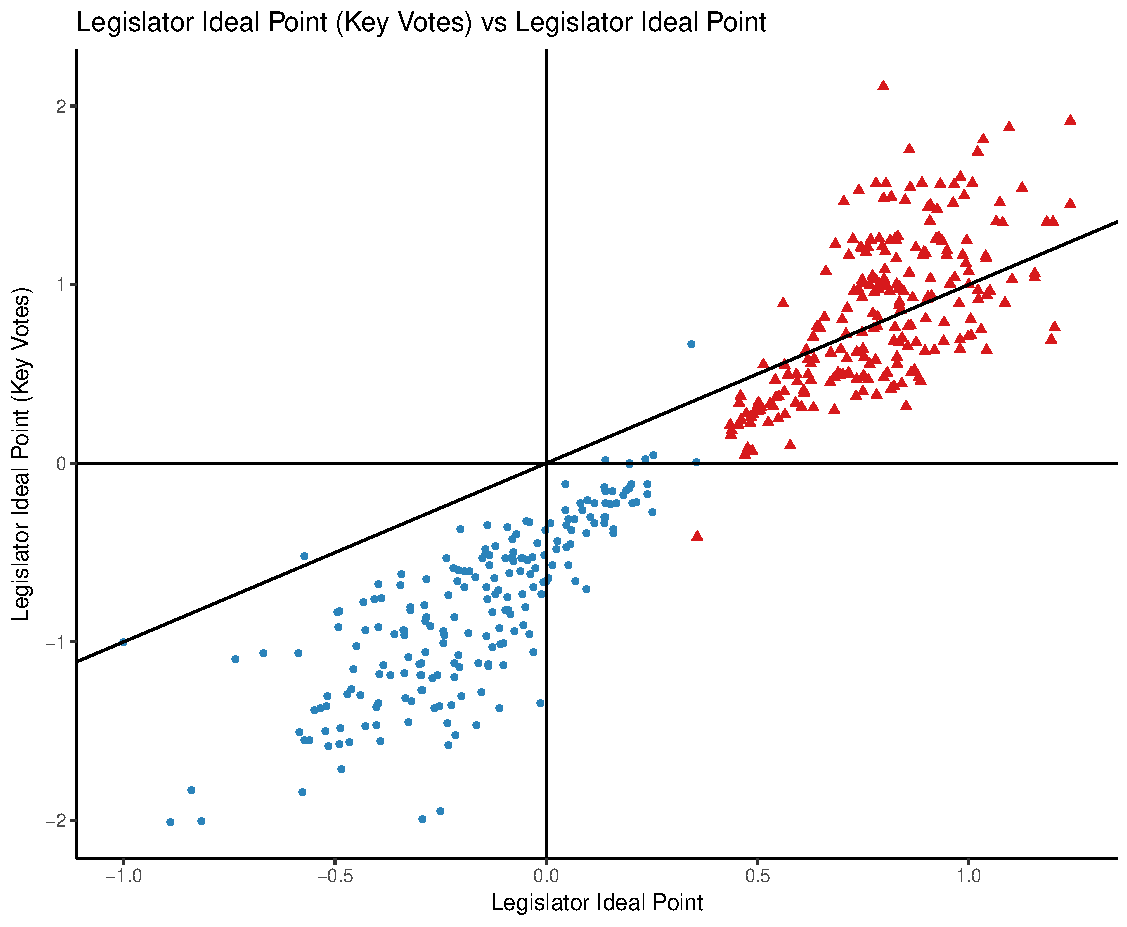
\includegraphics[width=.33\textwidth]{/Users/dsimp/GitHub/Clinton(2006)Rep/drafts/histogram/histo_change} \\
     & &  \\
    \small (D) District Mean Ideology &
    \small (E) Same-Party Mean Ideology &
    \small (F) Non-Same-Party Mean Ideology  \\
	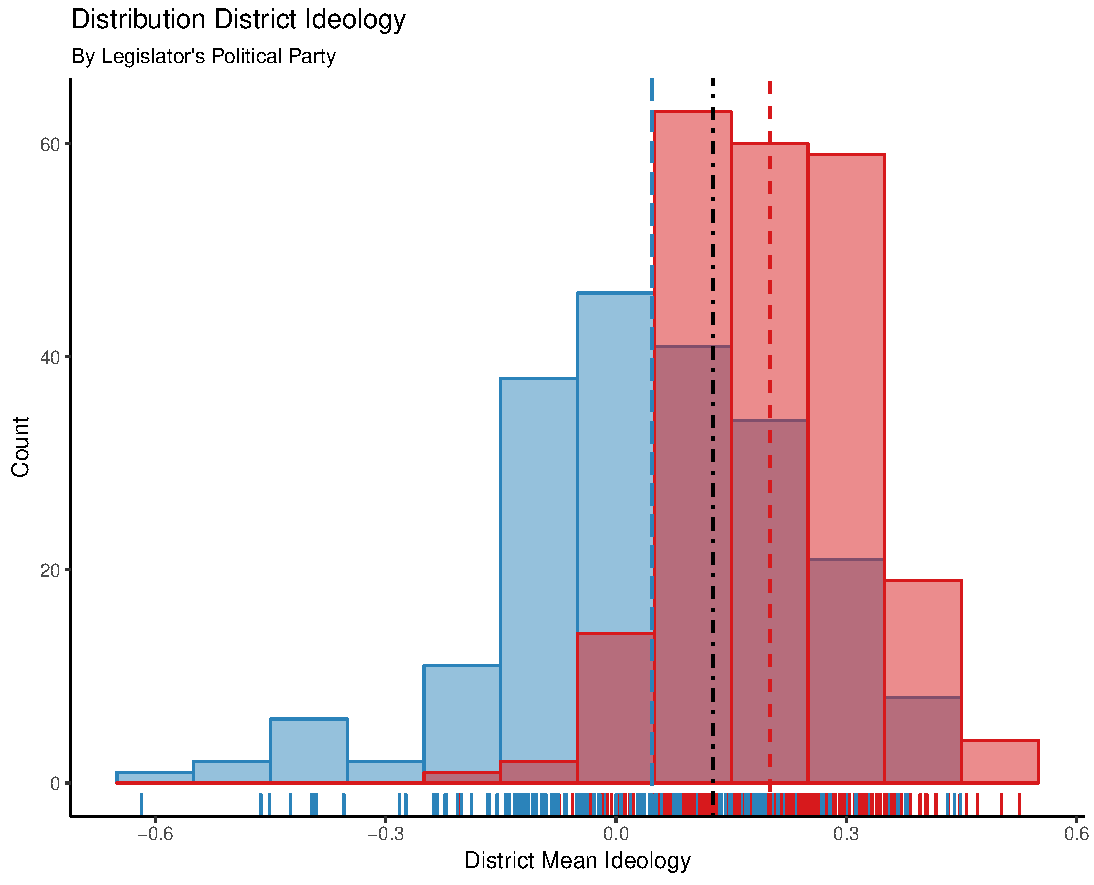
\includegraphics[width=.33\textwidth]{/Users/dsimp/GitHub/Clinton(2006)Rep/drafts/histogram/histogram-3} &
    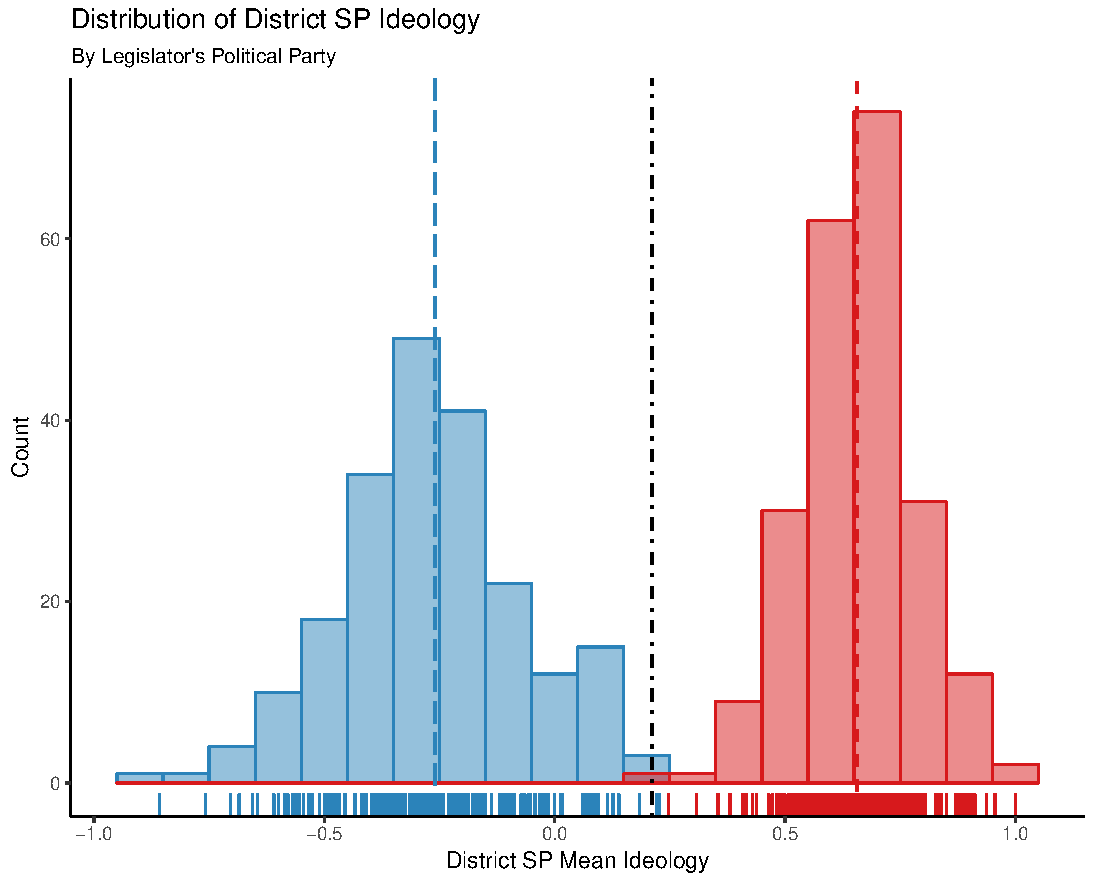
\includegraphics[width=.33\textwidth]{/Users/dsimp/GitHub/Clinton(2006)Rep/drafts/histogram/histogram-4} &
    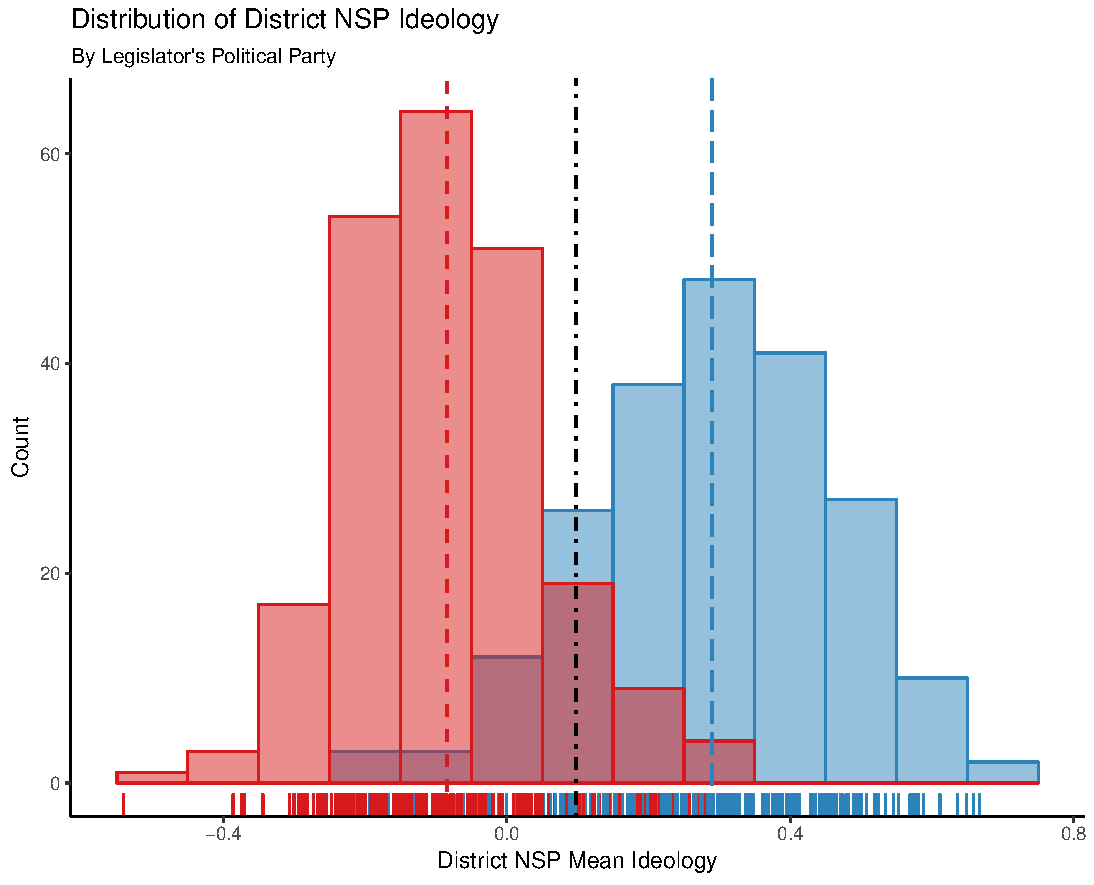
\includegraphics[width=.33\textwidth]{/Users/dsimp/GitHub/Clinton(2006)Rep/drafts/histogram/histogram-5} \\
      & &  \\
    \small (G) Opposite Party Mean Ideology&
    \small (H) Independent Mean Ideology&
    \small (I) Opposite Party vs Independent  \\
    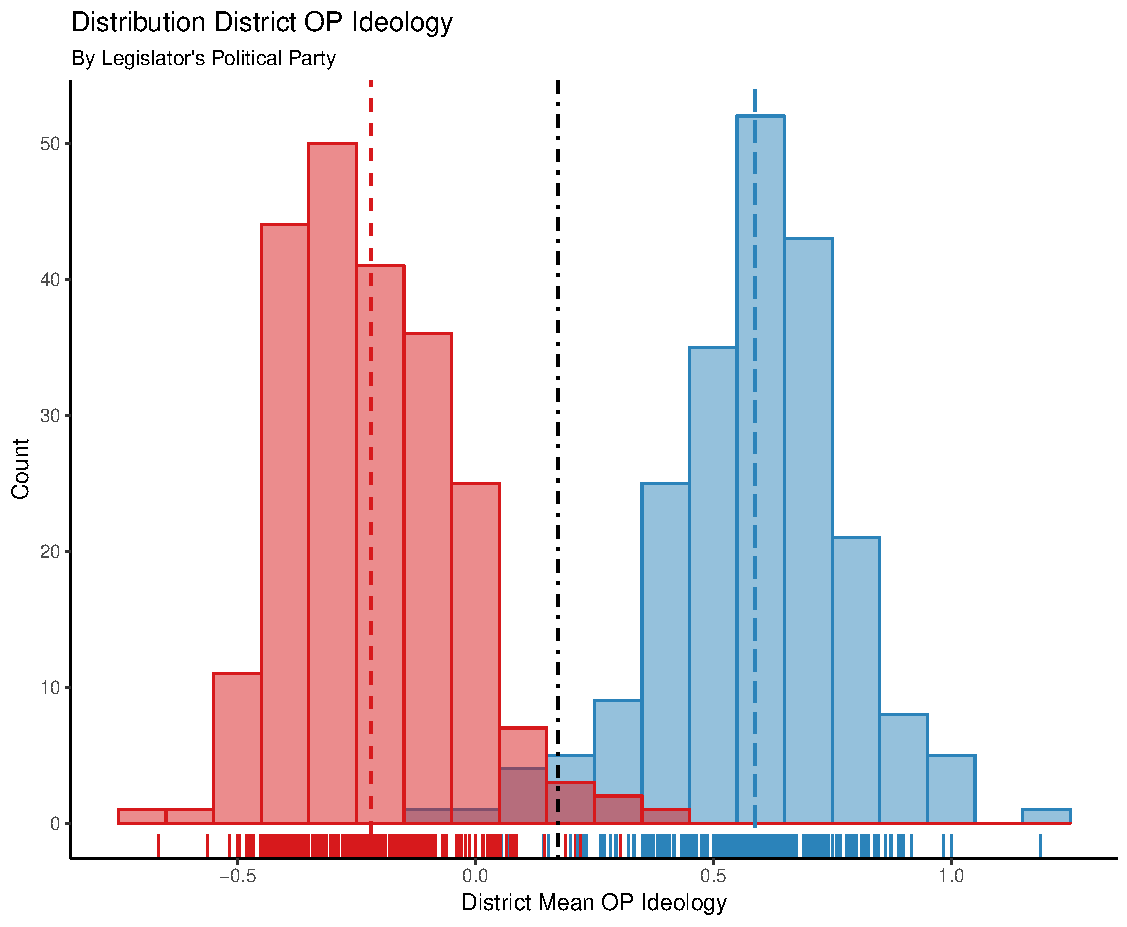
\includegraphics[width=.33\textwidth]{/Users/dsimp/GitHub/Clinton(2006)Rep/drafts/histogram/histogram-6} &
    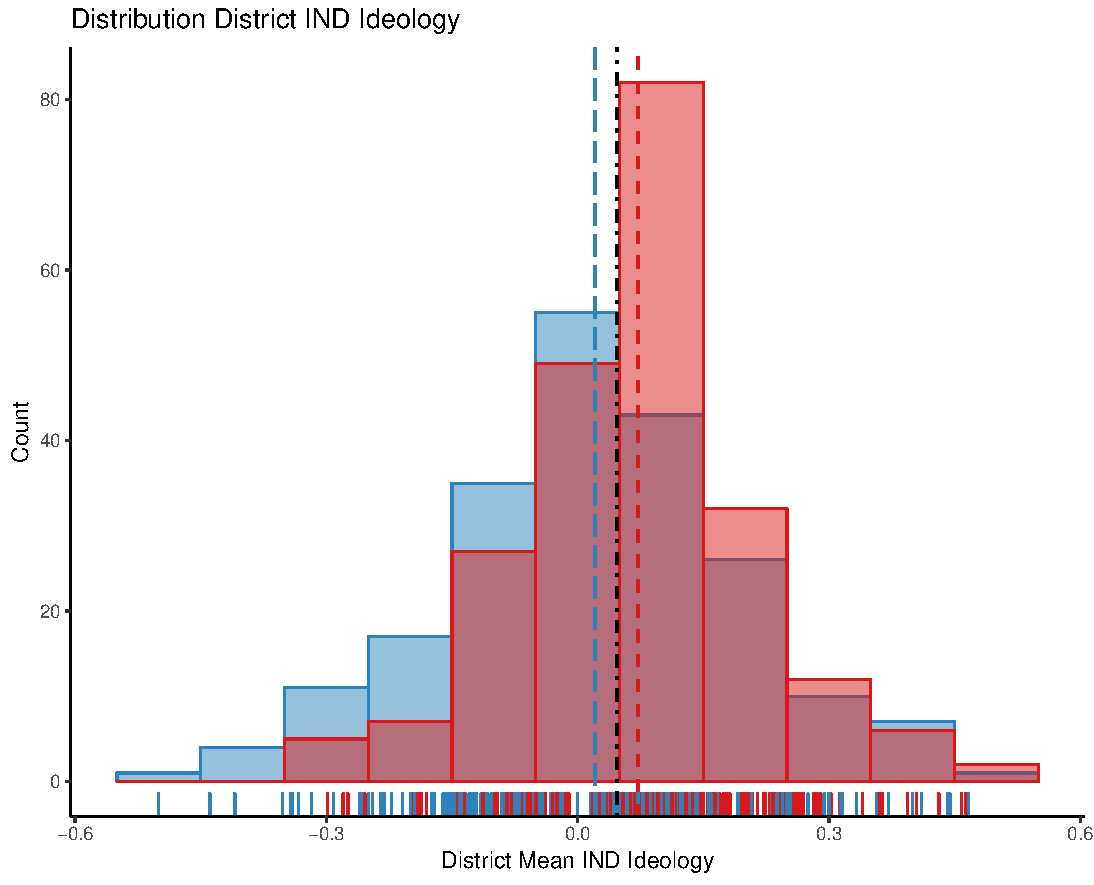
\includegraphics[width=.33\textwidth]{/Users/dsimp/GitHub/Clinton(2006)Rep/drafts/histogram/histogram-7} &
    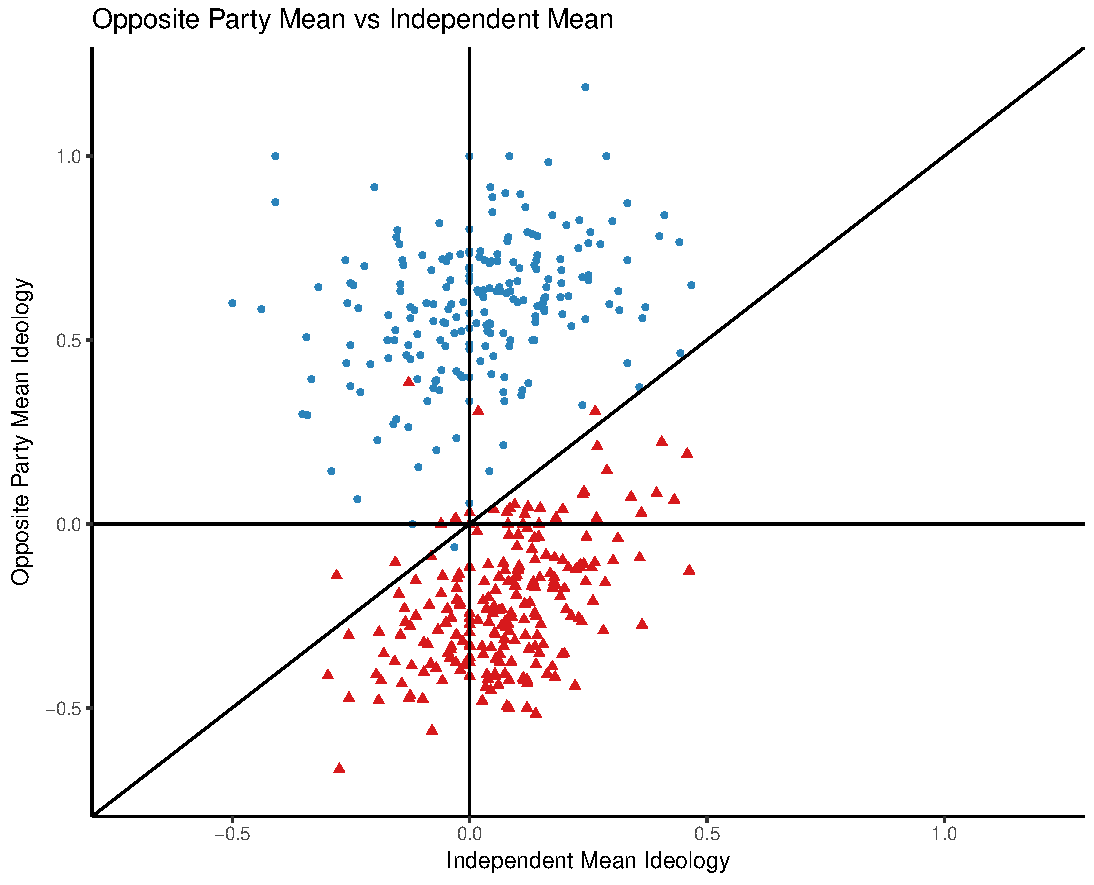
\includegraphics[width=.33\textwidth]{/Users/dsimp/GitHub/Clinton(2006)Rep/drafts/histogram/histo_diff} \\
       & &  \\
  \end{tabular}
    %}   
 \end{centering}\\
  \small \textbf{Note:} The histograms illustrate the distribution of legislator ideal points and sub-district constituency mean ideology grouped by legislator party. The red (blue) histograms provide the distributions in Republican (Democratic) held districts. For histograms, the short dashed lines are the Republican means, the long dashed line are the Democratic means, and the dotted and dashed line is the chamber mean. Plot (C) shows the change in district district ideal point when key votes are used instead of all votes. Points above (below) the 45-degree line are more conservative (liberal) when key votes are used. Plot (I) compares district independent mean ideology to district opposite party mean ideology. Members with points above (below) the 45-degree line have opposite party constituents more conservative (liberal) than their independent constituents. 
\end{figure}